\documentclass{beamer}
\usetheme{Boadilla}

\usepackage{amsmath}
\usepackage{amsfonts}
\usepackage{amssymb}
\usepackage{tikz}

\title{My Beamer Example}
\author{My Name}
\institute{My Home Institution}
% I normally would use \date{\today}. I wrote out the date instead so that if
%  you compile it on a different day it still looks like the example pdf
\date{June 2, 2017}

\begin{document}

	% Your first slide should always be a title slide
	\begin{frame}
		\maketitle
	\end{frame}
	
	\begin{frame}{Tables}
		Let's make a simple table for boolean logic.
		% We will start in the center environment to center our table
		\begin{center}
			% tabular takes an argument telling it how many columns and the formatting of the columns
			% c: center aligned column
			% l: left-aligned column
			% r: right-aligned column
			% placing a | (shift+\) places a verticle line in the table 
			%               in the same place relative to the columns
			\begin{tabular}{c|c||c|c}
				% Use & to tell tabular you are moving to the next
				%                                 column of your row
				X & Y & X AND Y & X OR Y \\
				% \hline makes a horizontal line at the top of your current row
				\hline
				T & T &    T    &    T   \\
				T & F     %% #1: Finish the table
			\end{tabular}
		\end{center}
		
		Matrices can be built in a similar manner, but you must be in math mode
		\begin{center}
			$
			% #2: Write down the matrix
			$
		\end{center}	
	\end{frame}	
	
	% the argument after the frame gives the slide a title
	\begin{frame}{Lists}	
		We can make an itemized list:
		\begin{itemize}
			\item This list
		        % #3: Finish this list
                \end{itemize}

		We can also make enumerated lists:
	        
                % #4: Write down the enumerated list with pauses in between each item

        \end{frame}
	
	
	% Add an argument to the frame environment to give your slide a title
	\begin{frame}{Definition Blocks}
	  
          % #5: Write down the definition block

		% the figure environment will center our picture, use internal logic to 
		% move it to a visually appealing place, make it easy to add a caption, 
		% and is often used in papers to more easily cite drawings and make a 
		% table of diagrams
		%     The [optional tag] is used to tell LaTeX where it should try to %      place the picture. h=here, t=top, b=bottom, etc.
		\begin{figure}[hb]
			% Use tikz to draw a right triangle
			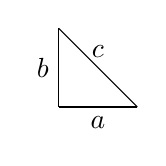
\begin{tikzpicture}
				%the node command here allows us to place a label along the line
				\draw (0,0) -- (1,0) node[midway, below] {$a$}; 
				\draw (0,0) -- (0,1) node[midway, left] {$b$};
				\draw (1,0) -- (0,1) node[midway, above] {$c$};
			\end{tikzpicture}
			\caption{A right triangle (No need to TeX this! Ola will explain how to use TikZ later)}
		\end{figure}
	\end{frame}
	

        % #6: TeX up the Theorems and Figures slide
	
	
	
	\begin{frame}{Advanced Topic- The Columns Environment}
		The columns environment splits your page up into multiple columns of content.
                
                \vspace{0.3in}

		% #7: TeX up the columns

                \vspace{0.3in}
			
		Columns is also a nice environment for placing equations and graphs side-by-side.		
	\end{frame}
	

\end{document}
